\documentclass{article}

% NeurIPS 2026 workshop template (as scaffolded by the project)
\usepackage[preprint]{neurips_2026}
\usepackage[utf8]{inputenc}
\usepackage[T1]{fontenc}
\usepackage{hyperref}
\usepackage{url}
\usepackage{booktabs}
\usepackage{amsfonts}
\usepackage{nicefrac}
\usepackage{microtype}
\usepackage{xcolor}
\usepackage{amsmath}
\usepackage{multirow}
\usepackage{graphicx}

\title{Exact Circulant-Block KRR on Regular-Grid Climate Fields: A CPU-Only Study}

\author{%
  Anonymous Author(s) \\
  \texttt{anon@example.org} \\
  % Affiliations omitted for double-blind review
}

\begin{document}

% Folded title/author block (space-saving: title kept verbatim; the
% \maketitle rule bars and the "Preprint." noticebox are omitted).
{\centering
{\Large\bfseries Exact Circulant-Block KRR on Regular-Grid Climate Fields:
A CPU-Only Study}\\[0.6ex]
Anonymous Author(s) \quad \texttt{anon@example.org}\par}
\vspace{1.4ex}

\noindent\textbf{Abstract.} We study exact kernel ridge regression (KRR) on
$H\times W$ regular-grid climate fields: the periodized (torus) kernel Gram
matrix is a block-circulant-with-circulant-blocks (BCCB) matrix, so
\emph{circulant-block embedding and FFT spectral shrinkage} give closed-form training/prediction at $O(N\log N)$ time /
$O(N)$ memory. We validate on \textbf{real data}: Kaplan SST v2 anomalies,
2005 monthly fields (1856-01..2023-01) on the $36\times72$ grid,
future-blind train 1856-01..2015-12 / test 2016-01..2022-12. The spectral
solve matches a dense floored-torus reference to $\sim\!10^{-12}$ relative
--- exact for the \emph{embedded-torus} kernel only; free-boundary gap 0.95
(matern32) / 0.12 (rbf). Masked reconstruction: matern32 RMSE 0.082--0.088
($\sim$14\% of field std 0.60). Contribution: a CPU-only circulant-block
implementation (78.7 s, 1.57 GB peak), a leakage-verified protocol, and a
resource-accounted real-data benchmark; the pre-registered transfer-forecast
claim is \textbf{REFUTED} (0/4); coverage violations disclosed per mask.

\section{Introduction}
\label{sec:intro}

Kernel ridge regression is a workhorse for spatial prediction in the
AI-for-climate toolbox \cite{ccai2026workshop}, but the $O(N^2)$ memory and
$O(N^3)$ time of the dense solve bound its use on gridded climate fields.
On \emph{regular grids}, circulant embedding \cite{dietrich1997fast,
wood1994statistical} and FFT spectral shrinkage keep the kernel solve exact
\emph{for the embedded (torus) kernel} \cite{gray2006toeplitz} (Section~\ref{sec:rel}).

We contribute a CPU-only implementation, a leakage-verified protocol, and a
resource-accounted real-data benchmark (Kaplan SST v2
\cite{kaplan1998analyses}); we claim no FFT-kernel,
spectral-regression, or ENSO-skill novelty; every number here is measured on
real Kaplan SST v2 --- never simulated.

\section{Related work}
\label{sec:rel}

\textbf{Structured and randomized kernel methods.} On regular grids the Gram
of a periodized kernel is BCCB, and circulant embedding underpins
\emph{exact} simulation of stationary Gaussian fields
\cite{dietrich1997fast,wood1994statistical}; we make the \emph{solve} exact
via FFT spectral shrinkage \cite{gray2006toeplitz}. Approximate alternatives trade exactness for
scale: random Fourier features (RFF) \cite{rahimi2007random}, Nystr\"om
\cite{williams2001using,drineas2005nystrom}, Fastfood \cite{le2013fastfood},
KISS-GP \cite{wilson2015kernel}, GPyTorch \cite{gardner2018gpyTorch},
spectral-GP \cite{lazaro2010sparse}, SPDE/INLA \cite{lindgren2011explicit}.
The closest sibling is an
\emph{approximate} sketch-circulant KRR on non-grid data
\cite{yin2019sketch}; exactness is verified against dense references
\cite{dietrich1997fast} (our P0 gate, Section~\ref{sec:p0}: $\sim\!10^{-12}$
relative).

\textbf{Uncertainty quantification for dependent data.} Split-conformal
intervals rest on exchangeability; for serially dependent residuals we
calibrate calendar-month blocks from the 60 terminal in-train years
(non-exchangeable conformal theory \cite{barber2023conformal},
dependent-data variant \cite{chernozhukov2018exact},
adaptive-conformal-inference (ACI) miscoverage updates
\cite{gibbs2021adaptive}).

\textbf{Significance for forecast comparisons.} Predictive-accuracy
comparisons on serially correlated errors use the Diebold--Mariano
statistic \cite{diebold1995comparing}, block resampling
\cite{kunsch1989jackknife}, and blocked cross-validation
\cite{bergmeir2012use,roberts2017crossvalidation,valavi2019blockcv};
with only 7 yearly test blocks we report a year-block bootstrap
MSE-difference CI instead of a Diebold--Mariano (DM)/HAC
(heteroskedasticity- and autocorrelation-consistent) statistic.

\textbf{ENSO forecasting baselines and ceilings.} Simple linear inverse
models \cite{penland1993prediction} and the operational multi-model
ensemble (NMME) skill record \cite{barnston2012skill,kirtman2014nmme}
bound what a single-model
transfer can claim, and the spring predictability barrier
\cite{webster1992monsoon} makes skill start-month-dependent; recent
deep/hybrid ENSO forecasters \cite{ham2019deep,zhou2022hybrid} are
GPU-scale. Our transfer arm (Section~\ref{sec:t3}) is a leakage-verified
\emph{benchmark protocol} against persistence, climatology and AR(1) --- not
an ENSO-forecasting contribution.

\section{Method: exact torus spectral KRR}
\label{sec:method}

\textbf{Embedding and training.} With circular row/column distances on the
$H\times W$ grid, a stationary kernel $k$ (Matern-3/2, RBF) yields a
\emph{BCCB} Gram matrix $K$ determined by its first column $c$,
diagonalized by the unitary 2D-DFT matrix $U$,
$K=U\,\mathrm{diag}(\hat{c})\,U^{*}$
\cite{gray2006toeplitz,dietrich1997fast}. Ridge regression
$\alpha=(K+\lambda I)^{-1}y$ reduces to
$\alpha=\mathcal{F}^{-1}_{2}\!\bigl(\mathcal{F}_{2}(y)/(\widehat{c}+\lambda)
\bigr)$ with $\widehat{c}=\mathcal{F}_{2}(c)$
--- two FFTs and one pointwise division, $O(N\log N)$ / $O(N)$; spectral
functionals use the same algebra (Section~\ref{sec:t2}).
\textbf{Spectral floor.} Non-torus kernels (RBF) give small negative BCCB
eigenvalues; floored at 0 (PSD projection).
\textbf{Torus exactness scope.} The BCCB Gram wraps the kernel across the
grid boundary, so this spectral solve is exact for the \emph{embedded-torus}
kernel, \emph{not} the free-boundary kernel; measured modeling gap per kernel
on a real test-window field: 0.95 (matern32) / 0.12 (rbf) relative.
\textbf{Masked
training.} For genuinely masked training we solve the exact free-boundary
system with preconditioned conjugate gradients (PCG; exact
block-Toeplitz-with-Toeplitz-blocks (BTTB) matvec via the
$(2N-1)$-mirror circulant,
preconditioned by the floored-torus spectral inverse; tol $10^{-8}$;
Section~\ref{sec:t1b}).

\section{Data and evaluation protocol}
\label{sec:data}

\textbf{Real data.} NOAA PSL Kaplan SST v2 monthly anomalies
\cite{kaplan1998analyses}: 2005 fields, 1856-01..2023-01, $36\times72$
(5$^\circ$) grid; netCDF-4 read with h5py; compute CPU-only
(NumPy/SciPy/scikit-learn). \textbf{Missing data.} 53.4\% of cells
carry the sentinel $-9.96921\times10^{36}$ and are treated as missing (100\%
polar caps rows 0--5, 30--35; 73\% high-N; 46\% high-S; 14.6\% tropics, land
columns): imputed by the valid-cell monthly mean for training, excluded from
\emph{every} evaluation target. \textbf{Valid-only evaluation.} Every metric
(RMSE, coverage, skill, correlation) uses \emph{valid cells only}:
denominators exclude imputed/missing cells --- coverage $=$ (valid
in-threshold)/(valid in subset), never diluted by the 53.4\% missing
mass; conformity likewise. \textbf{Splits.} Fields are 0-indexed from 1856-01 (index 0).
Future-blind: train $[0,1920)$ = 1856-01..2015-12; test $[1920,2004)$ =
2016-01..2022-12 (84 months); month 2004 (2023-01) excluded, so
$1920{+}84{+}1{=}2005$ fields in total.
\textbf{Protocol (leakage-verified).} (i) masked-cell holdout on the test
window: random 10/30/50\% and halo ($w{=}1/2/4$) masks (a halo mask is the
radius-$w$ neighborhood of the persistent missing regions: polar caps and
high-latitude strips); (ii)
calendar-month-block split-conformal intervals (construction in
Section~\ref{sec:t1a}), coverage diagnosed \emph{per mask} on global, seam
(2016--2017: the 24 test months at the train/test junction), and decay
(2016: its first 12 months, where imputation-boundary effects decay)
subsets, target 0.90
\cite{barber2023conformal,chernozhukov2018exact,gibbs2021adaptive}; (iii)
5-fold \emph{temporal-block} CV for the functional arm \cite{bergmeir2012use};
(iv) a future-blind forecast arm with a pre-registered win rule tested by
year-block bootstrap \cite{kunsch1989jackknife} (7 blocks 2016--2022, 2000
resamples, seed 7); DM/HAC
omitted at $n{=}7$ \cite{diebold1995comparing}; (v) pooled exact/Nystr\"om/RFF baselines
\cite{rahimi2007random,williams2001using,pedregosa2011scikit}.

\section{Experiments and results}
\label{sec:results}

\subsection{P0: torus exactness on a real field}
\label{sec:p0}
On a real test-window field (2016-01, index 1920, $\lambda{=}10^{-3}$) the
spectral solve matches the dense floored-torus reference to
$2.62\times10^{-12}$ (matern32) / $1.12\times10^{-12}$ (rbf) relative inf-norm
--- \textbf{PASS} at the $10^{-6}$ gate; torus-vs-free gap 0.95 / 0.12.

\subsection{Reconstruction under leakage-aware masks (T1a)}
\label{sec:t1a}
On the 84 test months ($\lambda{=}10^{-4}$; Table~\ref{tab:t1a}): matern32
RMSE 0.0816--0.0880 ($\sim$14\% of field
anomaly std 0.6001); rbf 0.2356--0.3155. Random-vs-halo gap
$+0.0040$ (random 30\% 0.0856 vs. halo $w{=}2$
0.0816). Coverage (target 0.90): matern32 global 0.877--0.898, rbf
0.816--0.893; violations disclosed individually: matern32 halo $w{=}2$ decay
0.747, halo $w{=}4$ seam 0.836 / decay 0.739; rbf halo $w{=}2$ global 0.816
(seam 0.837), halo $w{=}4$ global 0.824. \textbf{Conformal construction.}
Per kernel, conformity scores are $|$\emph{residual}$|$ on \emph{valid} cells
of the 60 terminal in-train fields of the same calendar month
(fields[1860:1920]); their 0.90 quantile is the per-month threshold;
$\lambda$ uses fields[1910:1920] only, test window untouched.

\begin{figure}[ht]
\centering
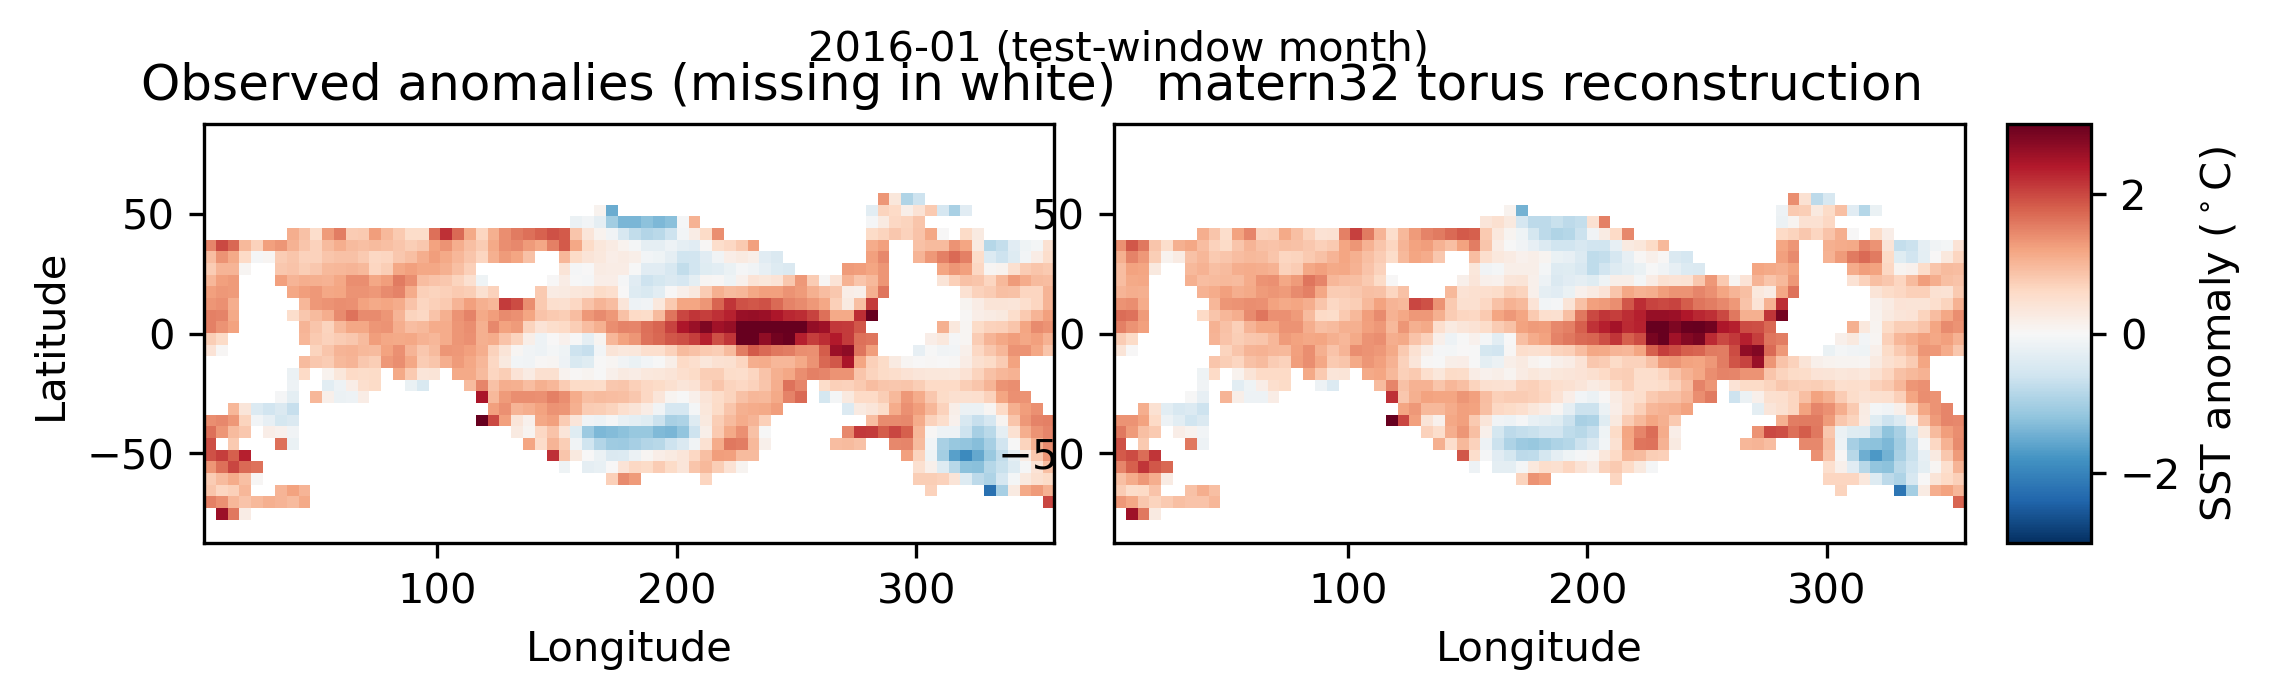
\includegraphics[width=0.32\linewidth]{figs/fig1_recon.png}
\caption{2016-01 test-window field: observed anomalies (missing cells in
white) vs.\ matern32 torus reconstruction ($\lambda{=}10^{-4}$,
Section~\ref{sec:t1a}).}
\label{fig:recon}
\end{figure}

\subsection{Genuinely masked training (T1b)}
\label{sec:t1b}
Exact free-boundary PCG (Section~\ref{sec:method}) at 10/30/50\% observed
converges to $10^{-8}$ in \emph{all} runs: mean iterations 245--281 (span
233--291), final relative residuals $4.69\times10^{-9}$--$9.81\times10^{-9}$,
masked RMSE 0.529--0.541; full-field T1a stays more accurate.

\subsection{Nino3.4 functional index (T2)}
\label{sec:t2}
The kernel-consistent functional (integral over the Nino3.4 box
\cite{trenberth1997definition} via $K(\cdot,\mathbf{1}_{\mathrm{box}})$) has
RMSE 0.0856 (corr 0.997) under 5-fold temporal-block CV over
all 2005 months, vs.\ 0.2696 for the direct ridge head on raw 2592-dim
features (3.2$\times$) and 0.7955 for the zero model. \textbf{Scope note:} a
leakage-safe \emph{method} comparison (2016--2022 participate as CV folds),
\emph{not} a future-blind forecast claim (Figure~\ref{fig:ts}).

\begin{figure}[ht]
\centering
\begin{minipage}[t]{0.28\linewidth}\centering
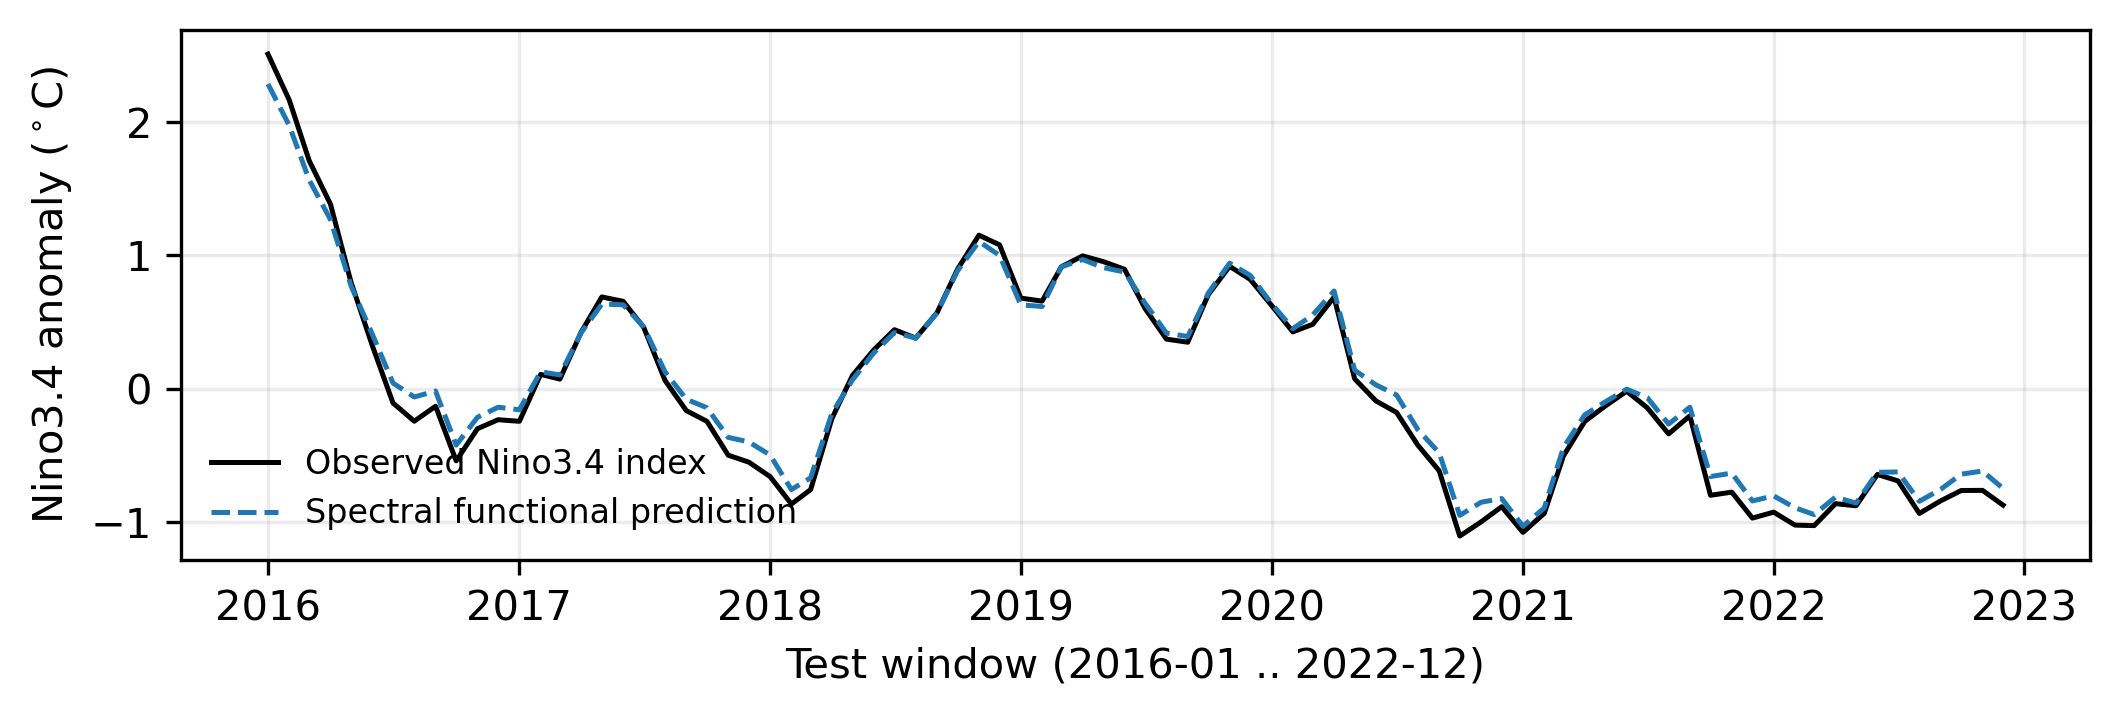
\includegraphics[width=\linewidth]{figs/fig2_nino34.png}
\end{minipage}\hfill
\begin{minipage}[t]{0.28\linewidth}\centering
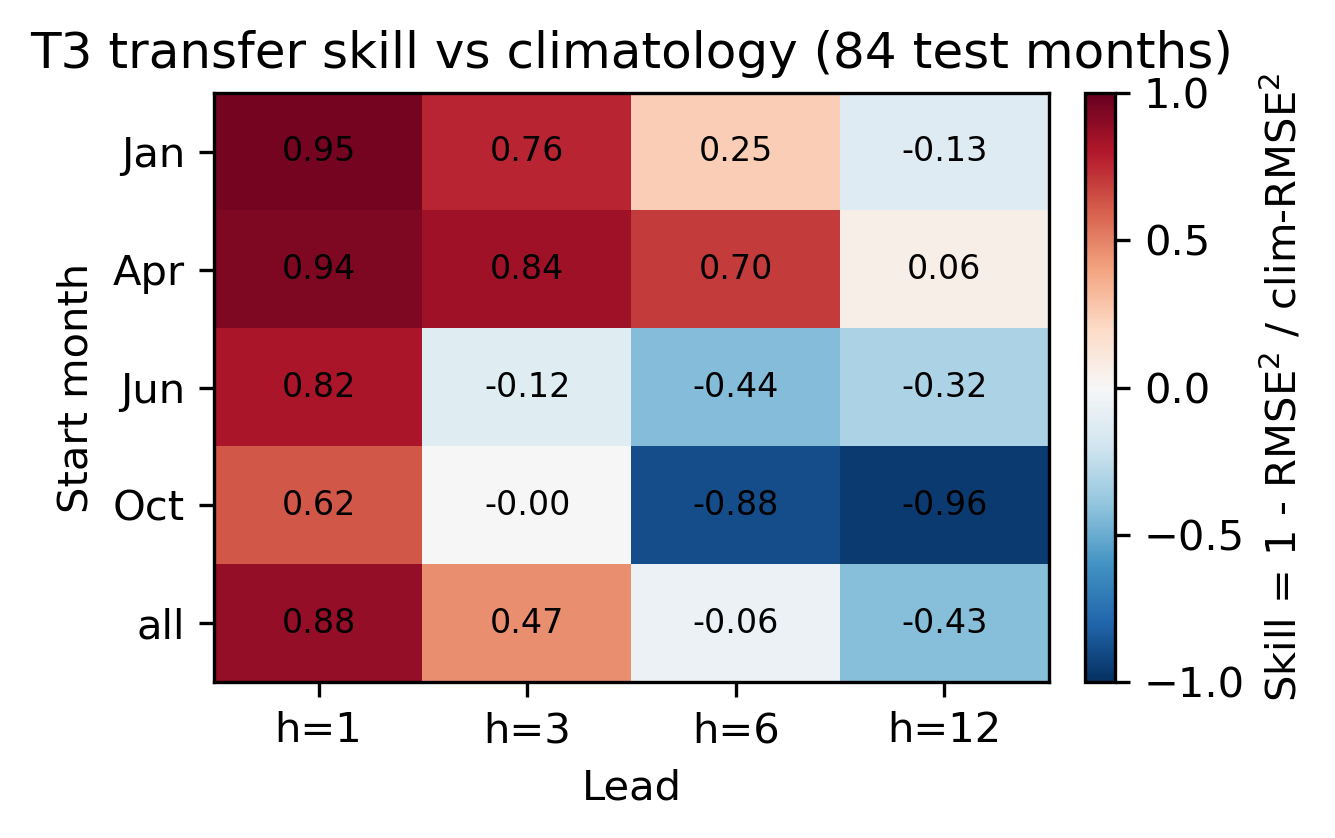
\includegraphics[width=\linewidth]{figs/fig3_skill.png}
\end{minipage}
\caption{Left: Nino3.4 index (observed) vs.\ spectral box-functional
prediction: the plotted curve is the 84-month test-window illustration of
the train-fit functional ($\lambda{=}10^{-2}$); the quoted RMSE 0.0856 /
corr 0.997 are the 5-fold temporal-block CV record over all 2005 months
(Section~\ref{sec:t2}). Right: T3 transfer skill vs.\ climatology by
start month and lead ($n{=}7$ per origin).}
\label{fig:ts}
\end{figure}

\subsection{Transfer forecast (T3): REFUTED under the pre-registered win rule}
\label{sec:t3}
Pre-registered win rule: \emph{supported} at $h$ iff transfer beats
persistence, climatology \emph{and} AR(1) in RMSE and skill with a
bootstrap-significant margin; \emph{refuted} if $>$ half fail.
\textbf{Aggregate verdict: REFUTED --- 0/4 horizons supported.} In
Table~\ref{tab:t3} (skill = MSSS $= 1-\mathrm{MSE}/\mathrm{MSE}_{\mathrm{clim}}$;
negative $=$ worse than train-only climatology), at $h{=}1$ the
transfer (0.268) loses to persistence (0.251) and AR(1) (0.241); at $h{=}3$
it loses to AR(1) (0.508); at $h{=}6$ it beats persistence (0.796 vs.\ 0.907)
but the MSE-difference CI includes zero ($p{=}0.234$, se 0.197); at $h{=}12$
skill is $-0.427$ (floor). \textbf{Minimum detectable margin.} With 7 year
blocks and 2000 draws, the bootstrap CI half-width (observed se 0.0056--0.333
across comparisons, vs-persistence 0.007--0.333) sets the minimum detectable
MSE margin; \emph{supported} requires the margin to exceed that half-width at
the 95\% level --- the closest margin, $h{=}1$, is $-0.0137$ (transfer
loses to AR(1)), not significant.
Truncation sweep (2012/2013/2014-12 cutoffs): $h{=}1$ skill 0.8795--0.8797.

Skill is origin-dependent (Table~\ref{tab:t3months},
Figure~\ref{fig:ts}): January best at $h{=}1$ (0.954); April strongest at
$h{\ge}3$ (0.84/0.70/0.06); October worst over
$h{=}1{,}6{,}12$ (0.62 / $-$0.00 / $-$0.88 / $-$0.96
across $h{=}1{,}3{,}6{,}12$; June worse at $h{=}3$); by
$h{=}12$ every origin is at or below the climatology floor --- only April
is marginally positive (0.059).

\subsection{Solve-cost control on a fixed pooled-cell task (B)}
\label{sec:b}
On the \emph{same} 2000 valid test cells, per-field spectral reconstruction
has pooled RMSE 0.0999; pooled exact/Nystr\"om/RFF KRR on (lat,lon)
coordinates reach 0.820--0.824 (Table~\ref{tab:ratio}). Coordinate-only
baselines sit at field-std level (zero 0.801 / global mean 0.605 / per-cell
climatology 0.813) --- a \emph{solve-cost control at a fixed task}, not an
end-to-end comparison.

\subsection{Resolution sensitivity (R) and scaling (S)}
2$\times$2 coarsening to 10$^\circ$ degrades reconstruction RMSE 0.0853 to
0.1667 (84 fields) and functional RMSE 0.0856 to 0.3825 (corr 0.997 to 0.950)
--- an honest negative. Fits are sub-ms through $N{=}10{,}368$
(0.0002--0.0005 s at $N{\in}\{1024,2592,10368\}$), $O(N\log N)$ flops /
$O(N)$ bytes; a 0.25$^\circ$ field ($N{=}1{,}036{,}800$ cells; one float64
field is 8.3 MB) fits in $\sim$0.04 GB --- the five working arrays of one
spectral solve: input field $y$, kernel first column $c$, rfft2 spectrum,
dual coefficients $\alpha$, and the pointwise $(\hat{c}{+}\lambda)$ buffer.
\textbf{Resources (CPU-only):} 78.7 s wall-clock, 1.57 GB peak RSS
(B dominates --- Nystr\"om-5000 at 29.8 s).

\begin{table}[ht]
\centering
\footnotesize
\begin{tabular}{lcccc}
\toprule
Mask & RMSE m32 & cov m32 & RMSE rbf & cov rbf \\
\midrule
random 10\%   & 0.0843 & 0.898 & 0.2525 & 0.873 \\
random 30\%   & 0.0856 & 0.892 & 0.2411 & 0.893 \\
random 50\%   & 0.0872 & 0.886 & 0.2356 & 0.892 \\
halo $w{=}1$  & 0.0827 & 0.896 & 0.2789 & 0.856 \\
halo $w{=}2$  & 0.0816 & 0.897 & 0.2839 & 0.816 \\
halo $w{=}4$  & 0.0880 & 0.877 & 0.3155 & 0.824 \\
\bottomrule
\end{tabular}
\caption{T1a (84 test months): masked-cell RMSE and coverage (target
0.90) per mask; violations in Section~\ref{sec:t1a}, none averaged.}
\label{tab:t1a}
\vspace{1.2ex}
\begin{tabular}{lccccc}
\toprule
$h$ & transfer & persistence & climatology & AR(1) & skill \\
\midrule
1  & 0.268 & 0.251 & 0.773 & 0.241 & 0.880 \\
3  & 0.565 & 0.562 & 0.773 & 0.508 & 0.466 \\
6  & 0.796 & 0.907 & 0.773 & 0.766 & $-0.061$ \\
12 & 0.923 & 1.154 & 0.773 & 0.879 & $-0.427$ \\
\bottomrule
\end{tabular}
\caption{T3 transfer RMSE by lead (84 test months; skill = MSSS vs.\
train-only climatology: 0.880/0.466/$-$0.061/$-$0.427; negative = worse
than climatology).\ \textbf{Verdict: REFUTED} --- 0/4 horizons.}
\label{tab:t3}
\vspace{1.2ex}
\begin{minipage}[t]{0.47\linewidth}
\centering
\begin{tabular}{lcccc}
\toprule
Origin & $h{=}1$ & $h{=}3$ & $h{=}6$ & $h{=}12$ \\
\midrule
Jan & 0.954 & 0.760 & 0.248 & $-0.126$ \\
Apr & 0.937 & 0.844 & 0.697 & 0.059 \\
Jun & 0.816 & $-0.120$ & $-0.437$ & $-0.318$ \\
Oct & 0.620 & $-0.001$ & $-0.884$ & $-0.955$ \\
\midrule
all & 0.880 & 0.466 & $-0.061$ & $-0.427$ \\
\bottomrule
\end{tabular}
\caption{T3 start-month $\times$ lead skill vs.\ climatology ($n{=}7$
per origin); at $h{=}12$ every origin is at or below the climatology floor
except April (+0.059).}
\label{tab:t3months}
\end{minipage}\hfill
\begin{minipage}[t]{0.47\linewidth}
\centering
\resizebox{\linewidth}{!}{%
\begin{tabular}{lccc}
\toprule
Method & RMSE & flop ratio & acc/flop (orders) \\
\midrule
spectral (2592)   & 0.0999 & 1         & --- \\
ridge $n{=}2000$  & 0.824  & $5.3\times10^4$ & 5.6 \\
ridge $n{=}4828$  & 0.820  & $7.5\times10^5$ & 6.8 \\
Nystr\"om $k{=}5000$ & 0.820 & $1.6\times10^6$ & 7.1 \\
RFF 5000          & 0.822  & $4.8\times10^2$ & 3.6 \\
\bottomrule
\end{tabular}}
\caption{B: pooled-cell RMSE (2000 cells) and solve cost vs.\ spectral;
acc/flop (orders) = $-{\log_{10}}$(accuracy-per-flop vs.\ spectral), so
higher = worse; baselines 0.801/0.605/0.813 --- solve-cost control on a
near signal-free task.}
\label{tab:ratio}
\end{minipage}
\end{table}

\section{Limitations and discussion}
\label{sec:limits}
(i) \textbf{Exactness is torus-embedded only}: free-boundary gap 0.95
(matern32) / 0.12 (rbf); masked
training falls back to PCG at $\sim$6$\times$ the T1a error. (ii)
\textbf{T3 transfer superiority is REFUTED} (0/4): 1-month skill reflects
autocorrelation already captured by persistence/AR(1); negative floor at
$h{=}12$; no transfer or ENSO-skill claim. (iii) \textbf{Coverage
is not uniform}: the reported-violation range on seam/decay subsets is
0.739--0.837 (over the reported $w{=}2$/$w{=}4$ halo masks: matern32
$w{=}4$ decay 0.739 / seam 0.836; rbf $w{=}2$ seam 0.837); all
violations reported, none averaged. (iv)
\textbf{Resolution sensitivity} is an honest negative (R/S above). (v)
\textbf{Kaplan smoothing caveat}: EOF-based reconstruction
\cite{kaplan1998analyses}; missing cells (53.4\%) imputed by monthly means,
excluded from all targets.

\section*{Conclusion}
Exact circulant-block KRR is a practical CPU-only route on regular grids:
torus-exact closed-form solves at $O(N\log N)$ / $O(N)$ (78.7 s / 1.57 GB);
masked reconstruction at $\sim$14\% of field std; the pre-registered
transfer claim is refuted, coverage violations and degradation reported
--- the contribution stands on implementation, protocol, benchmark, not
novelty.

\clearpage
{\footnotesize
\setlength{\bibsep}{0pt}
\setlength{\parskip}{0pt}
\setlength{\topsep}{0pt}
\setlength{\parsep}{0pt}
\bibliography{main}
\bibliographystyle{abbrv}
}

\end{document}